\documentclass[11pt]{article}
\usepackage[margin=1in]{geometry}
\usepackage{graphicx}
\usepackage{booktabs}
\usepackage{amsmath}
\usepackage{hyperref}
\usepackage{enumitem}
\title{Neural Stiff-Chemistry Surrogates in DeepFlame:\\Implementation Pitfalls, Coupled-Solver Safeguards, and Target Semantics for H$_2$ and C$_2$H$_4$}
\author{Project draft generated from experiment record}
\date{\today}

\begin{document}
\maketitle

\begin{abstract}
This draft manuscript summarizes the current state of an EFNO-oriented stiff-chemistry implementation and deployment program for H$_2$ and C$_2$H$_4$ inside DeepFlame. The strongest present story is not a final claim of solved CFD-coupled chemistry replacement, but an evidence chain showing: (1) EFNO-style stiff-chemistry surrogates are highly sensitive to implementation details, including a consequential transformed-state decode bug; (2) offline accuracy and rollout metrics do not directly predict coupled DeepFlame usefulness; (3) H$_2$ deployment requires thermodynamic diagnostics and guarded hybrid policies to remain solver-usable; and (4) for the more difficult C$_2$H$_4$ case, data construction and label semantics appear to dominate the remaining error budget. The manuscript is therefore organized as a reviewable partial-results paper with explicit negative results, deployment failures, and reproducible artifacts.
\end{abstract}

\section{Introduction}
Stiff chemistry surrogates are attractive for CFD because conventional chemistry integration remains expensive, but the deployment-facing evidence base for neural surrogates is still thin. This project targets a faithful EFNO-style implementation study for H$_2$ and C$_2$H$_4$ inside DeepFlame, with emphasis on what survives coupled deployment rather than only what looks good offline.

\section{Background and related work}
The manuscript is grounded in the EFNO paper by Weng et al. and a local-paper crosswalk covering data generation, augmentation, and coupled-validation issues from related combustion-chemistry learning papers. A recurring theme from both the literature and the present experiments is that model architecture alone is not decisive: data semantics, postprocessing contracts, and deployment diagnostics all materially affect conclusions.

\section{Reproducible workflow and software stack}
The implementation workflow combines PDF extraction and structured notes, DFODE-kit extensions for EFNO-style training and evaluation, and DeepFlame export bridges for MLP and FNO-like surrogates. All substantive experiments are documented in the project docs site together with scripts and artifact paths.

\section{Offline H$_2$ reproduction and implementation diagnosis}
The H$_2$ program established seeded offline baselines, rollout-aware EFNO-style training, and a key implementation diagnosis: a transformed-state species decode bug materially distorted rollout behavior. After correcting the update rule to act in the proper transformed state space, self-rollout behavior changed qualitatively and the corrected branch became a credible offline reference for deployment-facing work.

\section{DeepFlame-coupled H$_2$: from failure to guarded deployment}
The H$_2$ coupled study showed that export correctness and offline metrics are not enough. Coupled failures appeared first as HP reconstruction breakdowns, which led to hybrid fallback policies, frozen-temperature gating, and a logistic risk guard. Table~\ref{tab:h2-deployment-summary} summarizes representative operating points for the corrected branch. In the present evidence base, $650$~K gives the strongest long-horizon single-threshold retention, while the logistic risk guard at threshold $0.5$ provides a more safety-oriented mode with lower HP-failure exposure at some cost in learned participation.

\begin{table}[t]
\centering
\small
\caption{Selected H$_2$ coupled-deployment operating points for the corrected branch in DeepFlame.}
\label{tab:h2-deployment-summary}
\begin{tabular}{p{2.5cm}p{2.8cm}p{3.4cm}p{2.2cm}}
\toprule
Mode & Learned frac. at $2\times10^{-5}$ & Cum. fallback frac. at $2\times10^{-5}$ & First time $>95\%$ fallback \\
\midrule
FT550 & 0.000 & 0.516 & 1.4e-05 \\
FT600 & 0.081 & 0.373 & -- \\
FT650 & 0.294 & 0.361 & -- \\
FT650+risk@0.5 & 0.241 & 0.381 & -- \\
\bottomrule
\end{tabular}
\end{table}


The H$_2$ evidence supports a reviewable claim that deployment-facing chemistry surrogates require contract alignment and explicit thermodynamic safeguards, not just better offline loss values.

\section{C$_2$H$_4$ baseline establishment and runtime bridge diagnosis}
For C$_2$H$_4$, the program first established a trustworthy stock DeepFlame baseline, diagnosed reduced-rank GPU pitfalls, and repaired the FNO runtime bridge by batching inference. These steps were necessary before data-quality conclusions could be trusted: without them, runtime pathologies could masquerade as model deficiencies.

\section{C$_2$H$_4$ data semantics: what the current best model still gets wrong}
The strongest current C$_2$H$_4$ data result is a calibrated mixed dataset that combines the solver-aligned $dp100$ case-pair backbone with a moderate canonical augmentation component. This mixed model survives to $5\times10^{-6}$ and is substantially better than earlier baselines, but the best-model-vs-stock anatomy shows a structured residual failure: cooler active cells are over-driven, the hot bulk exhibits widespread source-term sign errors, and several late intermediates are still heavily suppressed.

\begin{figure}[t]
  \centering
  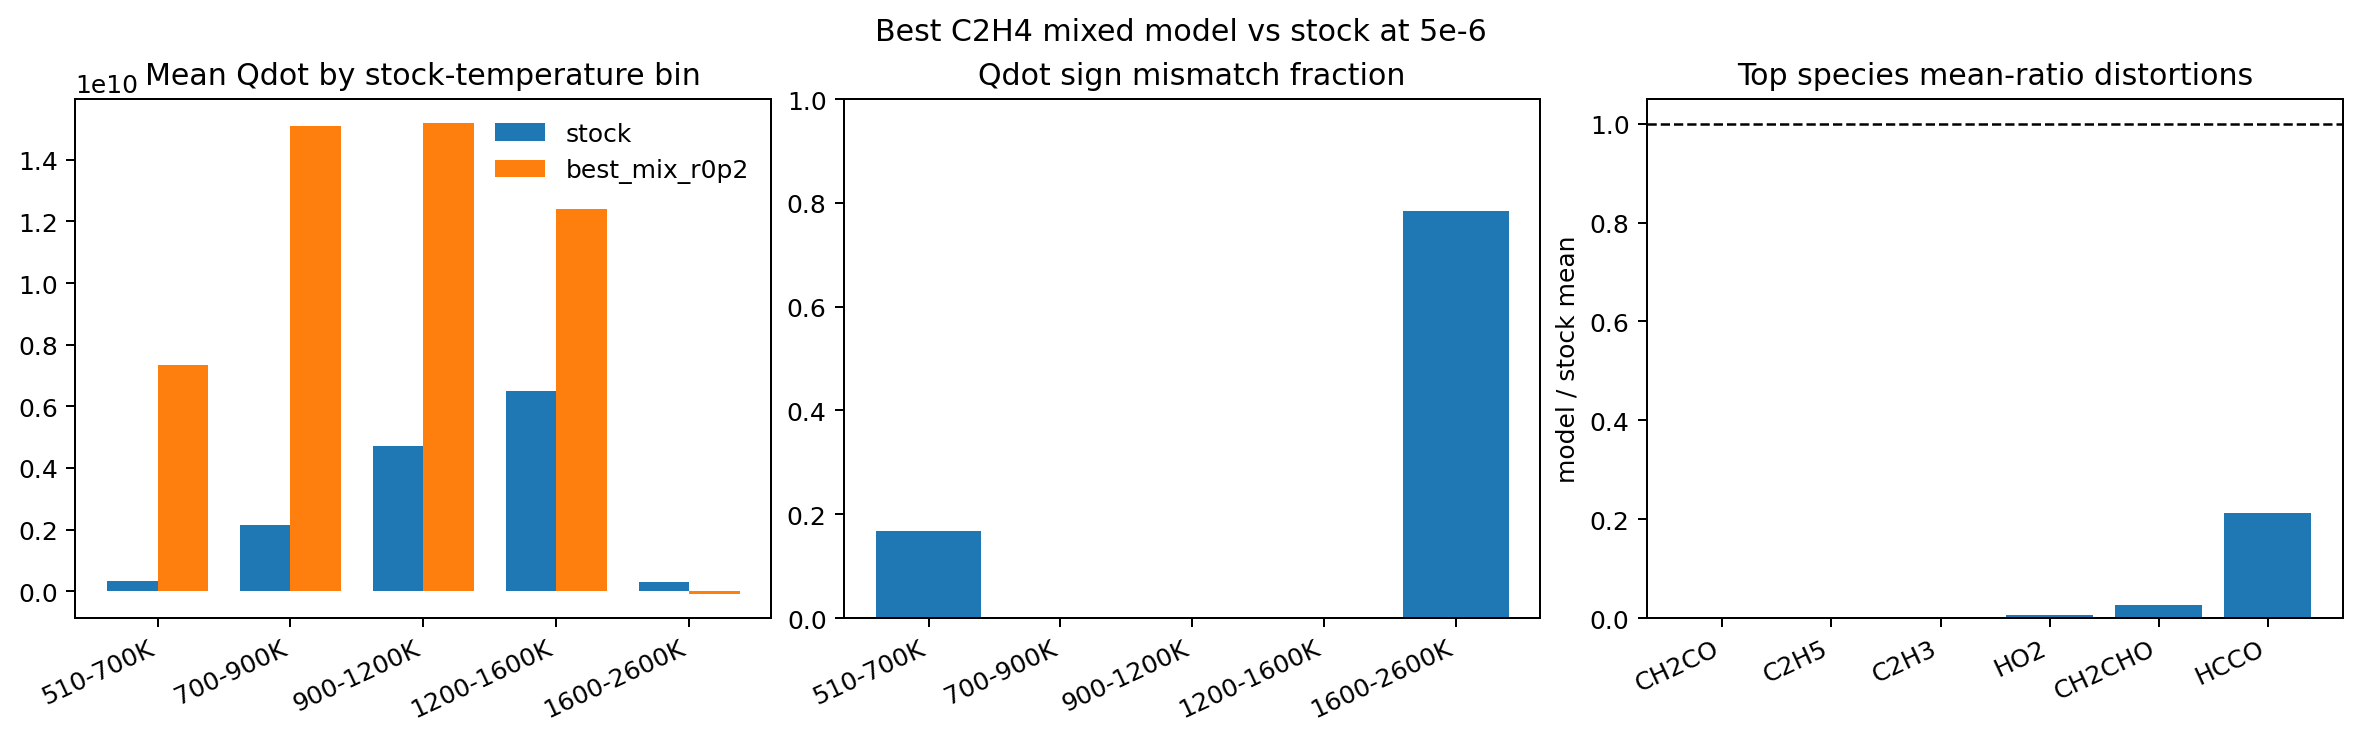
\includegraphics[width=0.95\linewidth]{../docs/findings/images/c2h4-bestmix-r0p2-vs-stock-5e-06.png}
  \caption{Matched-mesh comparison between the current best mixed C$_2$H$_4$ model and the stock DeepFlame baseline at $5\times10^{-6}$. The figure highlights temperature-binned source-term mismatch and the strongest mean-ratio species distortions.}
  \label{fig:c2h4-bestmix-vs-stock}
\end{figure}

The next diagnostic step showed that the target-semantics hypothesis is real in the data itself: one-step chemistry-proxy relabeling of case-pair current states produces materially different targets, especially on key intermediates. Table~\ref{tab:c2h4-error-anatomy} summarizes the most distorted active-region species in the current best mixed model, while Table~\ref{tab:c2h4-chemproxy-mismatch} shows that the original CFD next-state labels differ materially from chemistry-proxy relabels on a sampled subset. However, deployment tests also showed that semantics-only fixes are not enough in isolation. A tiny pure chemistry-proxy model fails catastrophically by $4\times10^{-7}$, while naive partial replacement of 10\% of labels preserves runtime survival but badly degrades solver-facing quality.

\begin{table}[t]
\centering
\small
\caption{C$_2$H$_4$ deployment-facing summary at $5\times10^{-6}$ for the stock baseline, the current best mixed model, and a naive partial chemistry-proxy relabeling ablation.}
\label{tab:c2h4-runtime-summary}
\begin{tabular}{p{3.1cm}rrrrr}
\toprule
Model & Mean $\dot{Q}$ & $\dot{Q}$/stock & $p_{\max}$ (Pa) & $T_{\min}$ (K) & mean $|\Delta T|$ (K) \\
\midrule
Stock DeepFlame & 1.62e+07 & 1.000 & 1.02e+05 & 499.249 & 0.828 \\
Best mixed ($dp100+canon@0.2$) & 2.51e+07 & 1.551 & 1.03e+05 & 499.159 & 0.927 \\
Partial chem-proxy (10\%) & -9.88e+08 & -60.952 & 1.03e+05 & 492.524 & 9.153 \\
\bottomrule
\end{tabular}
\end{table}

\begin{table}[t]
\centering
\small
\caption{Largest active-region species distortions for the current best mixed C$_2$H$_4$ model relative to stock at $5\times10^{-6}$.}
\label{tab:c2h4-error-anatomy}
\begin{tabular}{lrrr}
\toprule
Species & Stock mean & Model mean & Model/stock \\
\midrule
CH2CO & 2.12e-04 & 2.95e-17 & 1.39e-13 \\
C2H5 & 1.50e-05 & 2.22e-16 & 1.47e-11 \\
C2H3 & 5.81e-05 & 3.45e-10 & 5.95e-06 \\
HO2 & 5.46e-05 & 3.64e-07 & 0.007 \\
CH2CHO & 6.63e-06 & 1.77e-07 & 0.027 \\
HCCO & 6.01e-06 & 1.28e-06 & 0.212 \\
\bottomrule
\end{tabular}
\end{table}

\begin{table}[t]
\centering
\small
\caption{Largest mean-ratio shifts between original CFD next-state labels and chemistry-proxy relabels on a 5k-row C$_2$H$_4$ subset.}
\label{tab:c2h4-chemproxy-mismatch}
\begin{tabular}{lrrr}
\toprule
Species & Original next mean & Chemistry-proxy next mean & Chem/original \\
\midrule
HCCO & 3.82e-07 & 1.34e-05 & 35.146 \\
C2H5 & 5.13e-06 & 2.12e-07 & 0.041 \\
CH2CHO & 2.54e-06 & 1.08e-05 & 4.269 \\
CH2OH & 1.38e-06 & 5.13e-06 & 3.713 \\
C2H3 & 3.90e-05 & 1.03e-04 & 2.651 \\
CH2CO & 6.24e-05 & 1.64e-04 & 2.621 \\
\bottomrule
\end{tabular}
\end{table}


Table~\ref{tab:c2h4-runtime-summary} makes the current C$_2$H$_4$ claim boundary explicit. The best mixed model is reviewably better than prior baselines, but naive partial chemistry-proxy relabeling is not yet a deployment improvement. Tables~\ref{tab:c2h4-error-anatomy} and \ref{tab:c2h4-chemproxy-mismatch} sharpen the interpretation: the remaining gap is tied both to suppressed intermediate chemistry in deployment and to a measurable mismatch between full-CFD and chemistry-only target semantics. This supports the more specific forward hypothesis that semantics must be improved without losing the solver-relevant manifold.

\section{Discussion}
The present evidence supports several broader lessons. First, transformed-state implementation details can dominate empirical conclusions. Second, offline and deployment-facing evaluations can disagree substantially because of postprocessing and thermodynamic contract issues. Third, for the more difficult C$_2$H$_4$ case, the dominant remaining bottleneck appears to be target construction rather than another round of small architectural or mixing sweeps.

\section{Conclusion}
The current project state is strong enough for a reviewable partial-results paper. For H$_2$, corrected implementation plus guards yields a credible deployment story. For C$_2$H$_4$, the strongest current result is a calibrated mixed-data baseline together with a clear diagnosis that better target semantics are needed, but must be introduced without abandoning the solver-relevant state manifold. The central take-home message is that offline surrogate success is insufficient without deployment-aware validation and explicit thermodynamic diagnostics.

\section*{Immediate remaining tasks before submission}
\begin{enumerate}[leftmargin=1.5em]
  \item Add citations from the extracted EFNO notes and local related papers.
  \item Package at least one H$_2$ offline corrected-decode figure and one H$_2$ coupled-timeline figure.
  \item Expand the manuscript body from a structured skeleton into a fully referenced narrative.
  \item Replace naive semantics-only C$_2$H$_4$ relabeling with a more selective semantics-improvement experiment, or scope that step explicitly as future work.
\end{enumerate}

\end{document}
